\documentclass{article}
\usepackage{ae,aecompl}
\usepackage{todonotes}
\usepackage{chngcntr}
\usepackage{tikz-cd}
\usepackage{graphicx}
\graphicspath{ {./images/}}
\usepackage[all,cmtip]{xy}
\usepackage{amsmath, amscd}
\usepackage{amsthm}
\usepackage{amssymb}
\usepackage{amsfonts}
\usepackage{bm}
\usepackage{qsymbols}
\usepackage{latexsym}
\usepackage{mathrsfs}
\usepackage{mathtools}
\usepackage{cite}
\usepackage{color}
\usepackage{url}
\usepackage{enumerate}
\usepackage{verbatim}
\usepackage[draft=false, colorlinks=true]{hyperref}
\usepackage{pdfpages}
\usepackage[margin=1.2in]{geometry}
\usepackage{IEEEtrantools}

\usepackage{fancyhdr}


\usepackage[nameinlink]{cleveref}


\DeclareMathOperator*{\ac}{accept}
\DeclareMathOperator*{\amax}{argmax}
\DeclareMathOperator*{\amin}{argmin}
\DeclareMathOperator*{\Aut}{Aut}
\newcommand {\al}{{\alpha}}
\newcommand {\abs}[1]{{\left\lvert#1\right\rvert}}
\newcommand {\A}{{\mathcal{A}}}
\newcommand {\AM}{{\mathrm{AM}}}
\newcommand {\AMp}{{\AM_{p}^{X}\!(\Ri_\w)}}
\newcommand {\B}{{\mathcal{B}}}
\DeclareMathOperator*{\Be}{Bern}
\newcommand {\Br}{{\dot{B}}}
\newcommand {\Ba}{{\mathfrak{B}}}
\newcommand {\C}{{\mathbb C}}
\newcommand {\ce}{\mathrm{c}}
\newcommand {\Ce}{\mathrm{C}}
\newcommand {\Cc}{\mathrm{C_{c}}}
\newcommand {\Ccinf}{\mathrm{C_{c}^{\infty}}}
\DeclareMathOperator{\cov}{Cov}
\DeclareMathOperator{\DEV}{DEV}
\newcommand {\Di}{{\mathbb D}}
\newcommand {\dom}{\mathrm{dom}}
\newcommand{\dist}{\stackrel{\mathrm{dist}}{=}}
\newcommand {\ud}{\mathrm{d}}
\newcommand {\ue}{\mathrm{e}}
\newcommand {\eps}{\varepsilon}
\newcommand {\veps}{\varepsilon}
\newcommand {\vrho}{{\varrho}}
\newcommand {\E}{{\mathbb{E}}}
\newcommand {\Ec}{{\mathcal{E}}}
\newcommand {\Ell}{L}
\newcommand {\Ellp}{{L_{p}[0,1]}}
\newcommand {\Ellpprime}{{L_{p'}([0,1])}}
\newcommand {\Ellq}{{L_{q}([0,1])}}
\newcommand {\Ellqprime}{{L_{q'}([0,1])}}
\newcommand {\Ellr}{L^{r}}
\newcommand {\Ellone}{{L_{1}([0,1])}}
\newcommand{\Elltwo}{{L_{2}([0,1])}}
\newcommand{\Ellinfty}{L^{\infty}}
\newcommand{\Ellinftyc}{L_{\mathrm{c}}^{\infty}}
\newcommand{\exb}[1]{\exp\left\{#1\right\}}
\DeclareMathOperator*{\Ext}{Ext}
\newcommand{\F}{{\mathcal{F}}}
\newcommand{\Fe}{{\mathbb{F}}}
\newcommand{\G}{{\mathcal{G}}}
\newcommand{\HF}{\mathcal{H}_{\text{FIO}}^{1}(\Rd)}
\newcommand{\Hr}{H}
\newcommand{\HT}{\mathcal{H}}
\newcommand{\ui}{\mathrm{i}}
\newcommand{\I}{{I}}
\newcommand{\J}{{\mathcal{J}}}
\newcommand{\id}{{\mathrm{id}}}
\newcommand{\iid}{\stackrel{\mathclap{\normalfont\mbox{iid}}}{\sim}}
\newcommand{\im}{{\text{im }}}
\newcommand{\ind}{{\perp\!\!\!\perp}}
\DeclareMathOperator*{\Int}{int}
\newcommand{\intx}{{\overline{\int_{X}}}}
\newcommand{\inte}{{\overline{\int_{\E}}}}
\newcommand{\la}{\lambda}
\newcommand{\rb}{\rangle}
\newcommand{\lb}{{\langle}}
\newcommand{\La}{\Lambda}
\newcommand{\calL}{{\mathcal{L}}}
\newcommand{\lp}{{\mathcal{L}}^{p}}
\newcommand{\lpo}{{\overline{\mathcal{L}}^{p}\!}}
\newcommand{\Lpo}{{\overline{\Ell}^{p}\!}}
\newcommand{\M}{{\mathbf{M}}}
\newcommand{\Ma}{{\mathcal{M}}}
\newcommand{\N}{{{\mathbb N}}}
\newcommand{\Na}{{{\mathcal{N}}}}
\newcommand{\norm}[1]{\left\|#1\right\|}
\newcommand{\normm}[1]{{\left\vert\kern-0.25ex\left\vert\kern-0.25ex\left\vert #1 
    \right\vert\kern-0.25ex\right\vert\kern-0.25ex\right\vert}}
\newcommand{\Om}{{{\Omega}}}
\newcommand{\one}{{{\bf 1}}}
\newcommand{\pic}{\text{Pic }}
\newcommand{\ph}{{\varphi}}
\newcommand{\Pa}{{\mathbb{P}}}
\newcommand{\Po}{{\mathcal{P}}}
\newcommand{\Q}{{\mathbb{Q}}}
\newcommand{\R}{{\mathbb R}}
\newcommand{\Rd}{{\mathbb{R}^{d}}}
\DeclareMathOperator{\rej}{reject }
\newcommand{\Rn}{{\mathbb{R}^{n}}}
\newcommand{\cR}{{\mathcal{R}}}
\newcommand{\Rad}{{\mathrm{Rad}}}
\newcommand{\ran}{{\mathrm{ran}}}
\newcommand{\Ri}{{\mathrm{R}}}
\newcommand{\supp}{{\mathrm{supp}}}
\newcommand{\Se}{\mathrm{S}}
\newcommand{\Sp}{S^{*}(\Rn)}
\newcommand{\St}{{\mathrm{St}}}
\newcommand{\Sw}{\mathcal{S}}
\newcommand{\T}{{\mathcal{T}}}
\newcommand{\ta}{{\theta}}
\newcommand{\Ta}{{\Theta}}
\newcommand{\topp}{\stackrel{p}{\to}}
\newcommand{\todd}{\stackrel{d}{\to}}
\newcommand{\toL}[1]{\stackrel{L^{#1}}{\to}} 
\newcommand{\toas}{\stackrel{a.s.}{\to}}
\DeclareMathOperator{\V}{Var}
\newcommand {\w}{{\omega}}
\newcommand {\W}{{\mathrm{W}}}
\newcommand {\Wnp}{\text{$\mathrm{W}$\textsuperscript{$n,\!p$}}}
\newcommand {\Wnpeq}{\text{$\mathrm{W}$\textsuperscript{$n\!,\!p$}}}
\newcommand {\Wonep}{\text{$\mathrm{W}$\textsuperscript{$1,\!p$}}}
\newcommand {\Wonepeq}{\text{$\mathrm{W}$\textsuperscript{$1\!,\!p$}}}
\newcommand {\X}{{\mathcal{X}}}
\newcommand {\Z}{{{\mathbb Z}}}
\newcommand {\Za}{{\mathcal{Z}}}
\newcommand {\Zd}{{\Z[\sqrt{d}]}}
\newcommand {\vanish}[1]{\relax}

\newcommand {\wh}{\widehat}
\newcommand {\wt}{\widetilde}
\newcommand {\red}{\color{red}}

% Distributions
\newcommand{\normal}{\mathsf{N}}
\newcommand{\poi}{\mathsf{Poisson}}
\newcommand{\bern}{\mathsf{Bernoulli}}
\newcommand{\bin}{\mathsf{Binomal}}
\newcommand{\multi}{\mathsf{Multinomial}}
\newcommand{\Exp}{\mathsf{Exp}}



% put your command and environment definitions here




% some theorem environments
% remove "[theorem]" if you do not want them to use the same number sequence


  \newtheorem{thrm}{Theorem}
  \newtheorem{lemma}{Lemma}
  \newtheorem{prop}{Proposition}
  \newtheorem{cor}{Corollary}

  \newtheorem{conj}{Conjecture}
  \renewcommand{\theconj}{\Alph{conj}}  % numbered A, B, C etc

  \theoremstyle{definition}
  \newtheorem{defn}{Definition}
  \newtheorem{ex}{Example}
  \newtheorem{exs}{Examples}
  \newtheorem{question}{Question}
  \newtheorem{remark}{Remark}
  \newtheorem{notn}{Notation}
  \newtheorem{exer}{Exercise}




\title{STATS305A - Lecture 17}
\author{John Duchi\\ Scribed by Michael Howes}
\date{11/18/21}

\pagestyle{fancy}
\fancyhf{}
\rhead{STATS305A - Lecture 17}
\lhead{11/18/21}
\rfoot{Page \thepage}

\begin{document}
\maketitle
\tableofcontents

\section{The bootstrap}
Today we will discuss two new techniques, the bootstrap and M-estimators.
\subsection{Motivation}
Suppose we have an estimate $\wh{\beta}$ from some procedure. How can we get a handle on the sampling variability of $\wh{\beta}$? Two approaches are:
\begin{itemize}
    \item Make modelling assumptions such as $y=X\beta + \eps$ where $\eps \iid (0,\sigma^2)$.
    \item Use the variability in the sample $(X_i,Y_i)_{i=1}^n \iid P$.
\end{itemize}
The bootstrap is an example of the second approach. The bootstrap is due to our own Brad Efron (1979). The idea is if we define the \emph{emprical distribution} of a sample $(x_i,y_i)_{i=1}^n$ to be:
\[ \wh{P}=\frac{1}{n}\sum_{i=1}^n \one_{(x_i,y_i)}.\]
Then the idea of the bootstrap is that sampling from $\wh{P}$ should approximate sampling from the true distribution $P$. There are many ways to implement this idea.
\subsection{Resampling bootstrap}
The resampling bootstrap is the most commonly used form of the bootstrap. It is often what people mean when they refer to the bootstrap. The procedure is as follow. First pick a large number $B$ which will be the number of bootstrap resamples. For $b=1,2,\ldots, B$, do the following:
\begin{itemize}
    \item Draw a sample of size $n$ $(X^{*b},Y^{*b})$ from $\wh{P}$ where $n$ is the size of the original sample. This is done by drawing indices $i_1,i_2,\ldots, i_n$ from $[n]=\{1,\ldots,n\}$ uniformly at random with replacement and then setting $X^{*b} =(X_{i_1}, \ldots , X_{i_n})$ and $Y^{*b} = (Y_{i_1},\ldots, Y_{i_n}).$
    \item  Then calculate $\wh{\beta}^{*b} = \wh{\beta}(X^{*b},Y^{*b})$ from the bootstrap resample.
\end{itemize}
We can then use $(\wh{\beta}^{*b})_{b=1}^B$ tp estimate the sampling distribution of $\wh{\beta}$ when we draw $(X,Y) \iid P$. There are two forms of error in this approximation:
\begin{itemize}
    \item There is error from the Monte-Carlo sampling. This can be reduced by increasing $B$ which should also be taken as large as computationally possible.
    \item There is also error because $\wh{P}\neq P$. This error cannot be eliminated.
\end{itemize}
\subsection{Theory of the bootstrap} 
How can one mathematically describe the ``success'' of the bootstrap? Suppose we have a parameter of interest $\ta \in \R$ and we are interested in an estimator $\wh{\ta}$. For example we may have $\wh{\ta}=c^T\wh{\beta}$ or $\wh{\ta}=\wh{\beta}_j$ or $\wh{\ta}=\Vert \wh{\beta}\Vert_2^2$. Define 
\[J_n(t,P) = \Pa(\sqrt{n}(\wh{\ta}_n - \ta^*)\le t),\]
where $\wh{\ta}_n = \wh{\ta}(X_1,\ldots, X_n ; Y_1,\ldots, Y_n)$ is an estimate calculated on an i.i.d. sample drawn from $P$ and $\ta^*$ is the population parameter. The function $J_n$ is the (normalized) CDF of the sampling distribution of $\wh{\ta}_n$ about $\ta^*$. We can similarly define 
\[J_n(t,\wh{P}) = \Pa(\sqrt{n}(\wh{\ta}^*_n - \wh{\ta}_n)\le t),\]
where $\wh{\ta}_n^* = \wh{\ta}(X^*,Y^*)$ where $(X^*,Y^*)$ is an i.i.d. sample of size $n$ from $\wh{P}$ (that is $(X^*,Y^*)$ is a bootstrap sample). Note that for the distribution $\wh{P}$, $\wh{\ta}_n$ is the population parameter. This is why we are now centring at $\wh{\ta}_n$. We call $J_n(t,\wh{P})$ the bootstrap CDF of the statistic $\wh{\ta}_n$. 

While calculating or approximating $J_n(t,P)$ maybe be very hard, we can always get a handle on $J_n(t,\wh{P})$ by drawing more bootstrap samples. Under some regularity conditions with have that with probability 1,
\[\sup_{t \in \R} \abs{J_n(t,P)-J_n(t,\wh{P})} \stackrel{n}{\longrightarrow} 0.\]
So for large $n$, $J_n(t,\wh{P})$ is close to $J_n(t, P)$. It can shown that under some assumptions the rate of convergence is $\sqrt{\frac{\log n}{n}}$. We thus have a picture that looks like the one below. The bootstrap density of $\wh{\ta}^*$ is close to the true density of $\wh{\ta}$. 

\begin{center}
    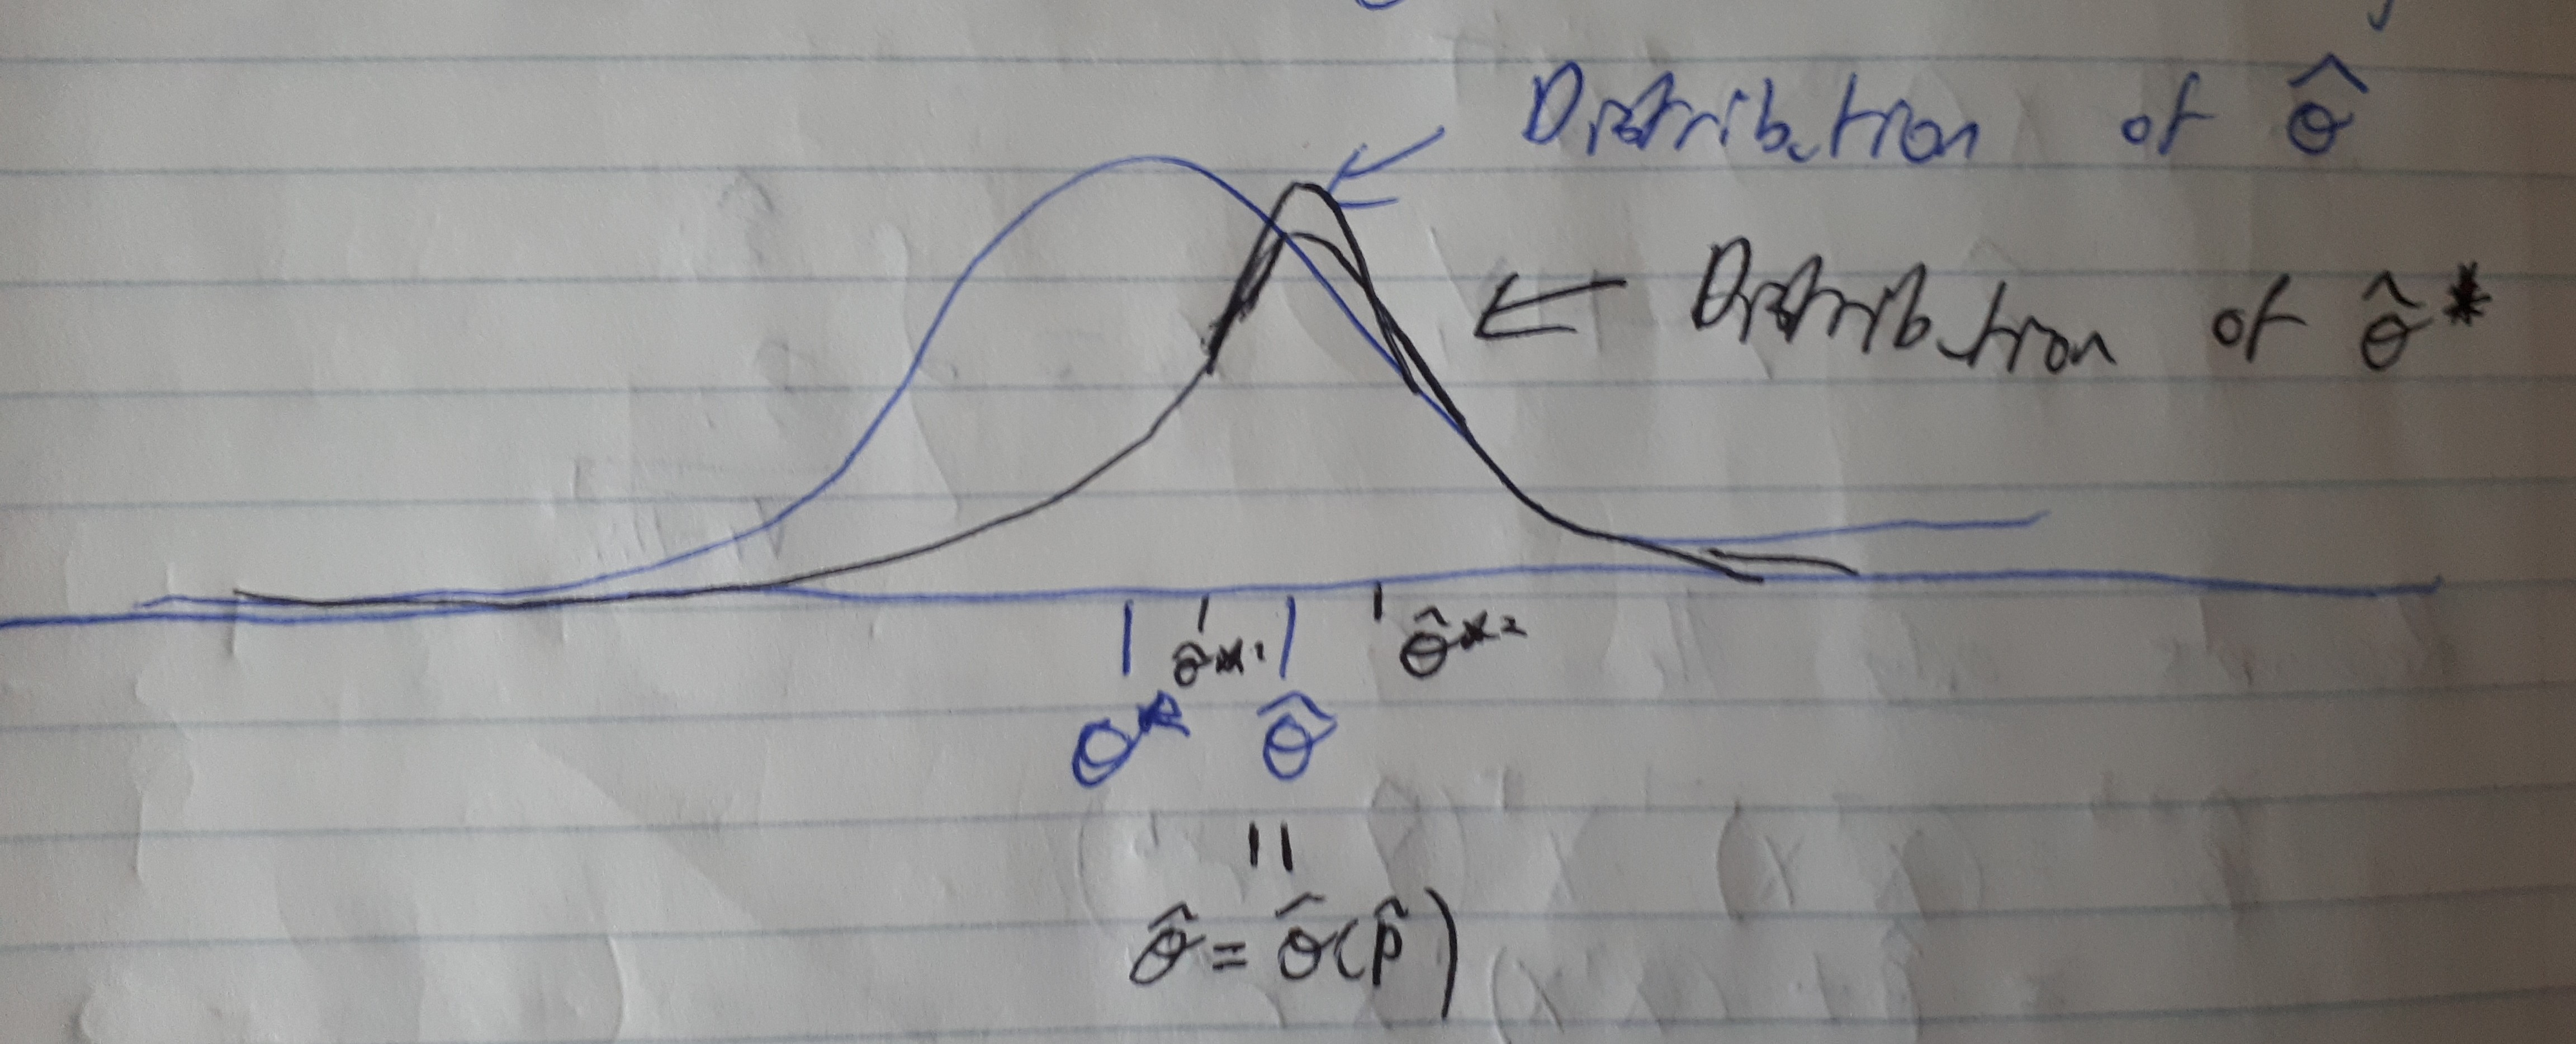
\includegraphics[width = 0.7\textwidth]{11_18_P01.jpg}
\end{center}

We can  use the bootstrap to define $1-\al$ confidence intervals for parameters $\ta \in \R$. One option is 
\[CI_\al = \left[\text{Quantile}_{\al/2}(\wh{\ta}^{*b}),\text{Quantile}_{1-\al/2}(\wh{\ta}^{*b})\right].\]
Another option is 
\[CI_\al' = \wh{\ta}\pm z_{1-\frac{\al}{2}}\sqrt{\V(\wh{\ta}^{*b}|\wh{P})},\]
where $z_{1-\frac{\al}{2}}$ is the $1-\frac{\al}{2}$ quartile of the standard normal. One can show that 
\[\Pa(\ta^* \in CI_\al), \Pa(\ta^* \in CI_\al') \stackrel{n}{\longrightarrow} 1-\al. \]
\subsection{The bootstrap in linear models}
One variant of the bootstrap is called the \emph{parametric bootstrap} which can be used if one has faith in their model. The procedure is as follows. In the linear model $y=X\beta +\eps$,
\begin{itemize}
    \item Fit model $\wh{\beta}$ based on original sample.
    \item Resample from the distribution $\wh{\beta}$ defines in the linear model ie $y^* =X\wh{\beta}+\eps^*$ but only resample the residuals.
    \item To resample the residuals, let $H=X(X^TX)^{-1}X^T$, $\wh{\eps}=Y-HY$ and $r_i = \wh{\eps}_i$ or $r_i = \frac{\wh{\eps}_i}{\sqrt{1-H_{ii}}}$ (both are used in practice). 
    \item Generate bootstrap resamples by resampling \emph{only} $r_i$ to get $r_i^{*b}$. Our bootstrap resample of $\wh{\beta}$ is then 
    \[\wh{\beta}^{*b} = (X^TX)^{-1}X^T(y+r^{*b})=\wh{\beta}+(X^TX)^{-1}X^Tr^{*b}. \]
\end{itemize}
We can then use the bootstrap resamples $\wh{\beta}^{*b}$ as described above. Some pros of this method are:
\begin{itemize}
    \item It works well when we have a fixed design matrix $X$.
    \item It is more efficient provided the model is true.
\end{itemize}
A major drawback is:
\begin{itemize}
    \item It really relies on the model assumptions. It especially relies on the noise being homeskedastic. Problems occur if $\E[\eps_i^2]=\sigma_i^2 \neq \sigma_j^2 = \E[\eps_j^2]$.
\end{itemize}
Thus people often use the \emph{non-parametric bootstrap} for the linear model which does not have the above drawback. Here we resample from $\wh{P}$ to get bootstrap resamples $(X^{*b}, y^{*b})$ and then we calculate
\[\wh{\beta}^{*b} = ((X^{*b})^TX^{*b})^{-1}(X^{*b})^Ty^{*b}.\]
This doesn't rely on the model being true and it allows from non homeskedastic noise. There is a drawback that for small sample sizes, the matrix $X^{*b}$ may be rank deficient but for reasonably large $n$, this does not happen often.
\subsection{Weighted bootstrap}
This is sometimes called Bayesian bootstrap although it isn't really Bayesian at all. We first fix a distribution $W$ which is supported on $[0,\infty)$ and satisfies $\E[W]=1$ and $\V[W]<\infty$. Often people use the exponetial distribution with scale 1.

At every bootstrap iteration $b$, we sample weights $w_1^{*b},\ldots, w_n^{*b} \iid W$. We then define a distribution based on these weights and our observed sample $(x_i,y_i)_{i=1}^n$, 
\[\wh{P}^{*b} =\frac{\sum_{i=1}^n w_i^{*b}\one_{(x_i,y_i)}}{\sum_{i=1}^n}. \]
We then define 
\begin{align*}
    \wh{\beta}^{*b} &=\amin_{c \in \R^d}\E_{\wh{P}^{*b}}\left[\norm{y-X^Tc}_2^2\right]\\
    &=\amin_{c \in \R^d} \frac{\sum_{i=1}^n w_i^{*b}(y_i-x_i^Tc)^2}{\sum_{i=1}^n w_i^{*b}}\\
    &= (X^T\diag(w_i^{*b})X)^{-1}X^T\diag(w_i^{*b})y.
\end{align*} 
There are similar asymptotic results for the weighted bootstrap as there are for the resampling bootstrap.
\section{M-estimators and robust regression}
Suppose we want to fit a regression $y_i = x_i^T\beta +\eps_i$ but maybe we no longer have $\eps_i \sim \Na(0,\sigma^2)$. Maybe there are some outlying $y_i$'s that are much larger than we'd expect for normally distributed errors.

For a histrical example, imagine trying to predict phone call length from distance to family. We might expect that the further apart two people are, the less often they would catch up and so their phone calls would be longer. The resulting would look something like this:

\begin{center}
    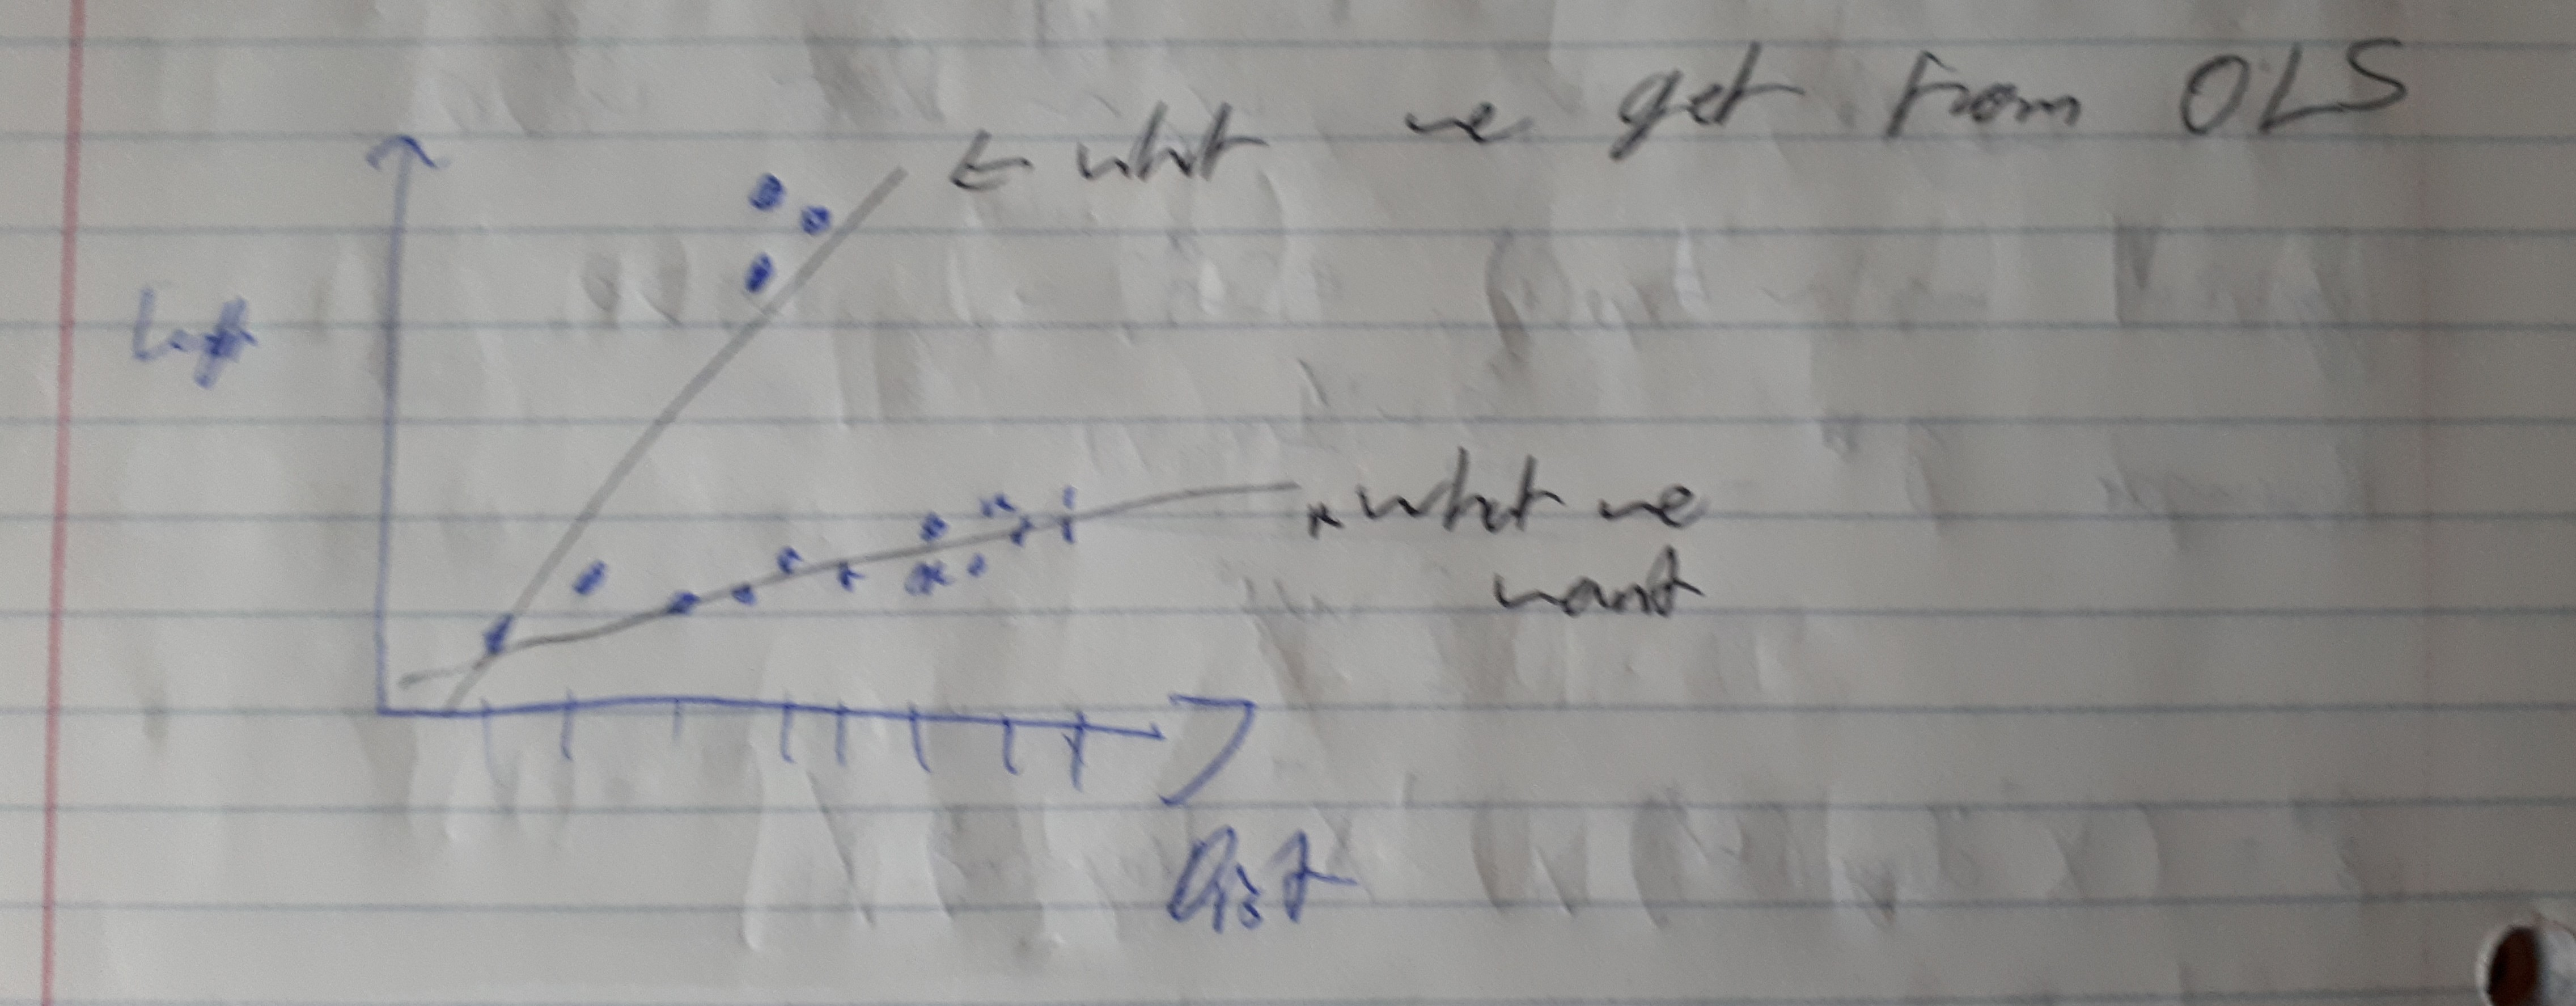
\includegraphics[width = 0.8\textwidth]{11_18_P02.jpg}
\end{center}
There is a problem because there are some people who just really likedtalking on the phone for a long time. These data points really mess up the linear model. Some solutions are:
\begin{itemize}
    \item Remove outliers. This can be hard as it is not always clear what make something an outlier.
    \item Choose an alternative to squared error to use when fitting (Huber, 70s-90s).
\end{itemize}
We will discuss the second approach.
\begin{defn}
    A \emph{loss function} is a function $l : \R \to \R^+$. We will sometimes require that $l(0)=0$.
\end{defn}
\begin{defn}
    Given data $(x_i,y_i)_{i=1}^n$ and a loss function $l$, the \emph{M-estimator} for predicting $Y$ from $X$ is the linear estimator $\wh{f}(x) = x^T\wh{\beta}$ where 
    \[\wh{\beta} = \amin_b \frac{1}{n}\sum_{i=1}^n l(y_i-x_i^Tb).\]
\end{defn}
The rough recipe is to choose a loss to capture properties we want the predictor to have. For example if $Y= f(X)+\eps$, then we might want 
\[\amin_t \E[l(Y-t)|X=x]=f(x).\]
For example for when $l$ is squared error we get the conditional mean above and when $l$ is absolute error we get the conditional median. Some examples of loss functions are:
\begin{itemize}
    \item \emph{Absolute error loss}: $l(t)=\abs{t}$. As stated above this has the property that \[\amin_t \E[\abs{Y-t}]=\text{median}(Y).\]
    \item \emph{$\eps$-insensitive loss}: If we don't care about if the predicted value is off by less than $\eps$ we can use the loss\[ l^\eps(t) = (t-\eps)_++(-t-\eps)_+.\] This loss looks like the black function
    \begin{center}
        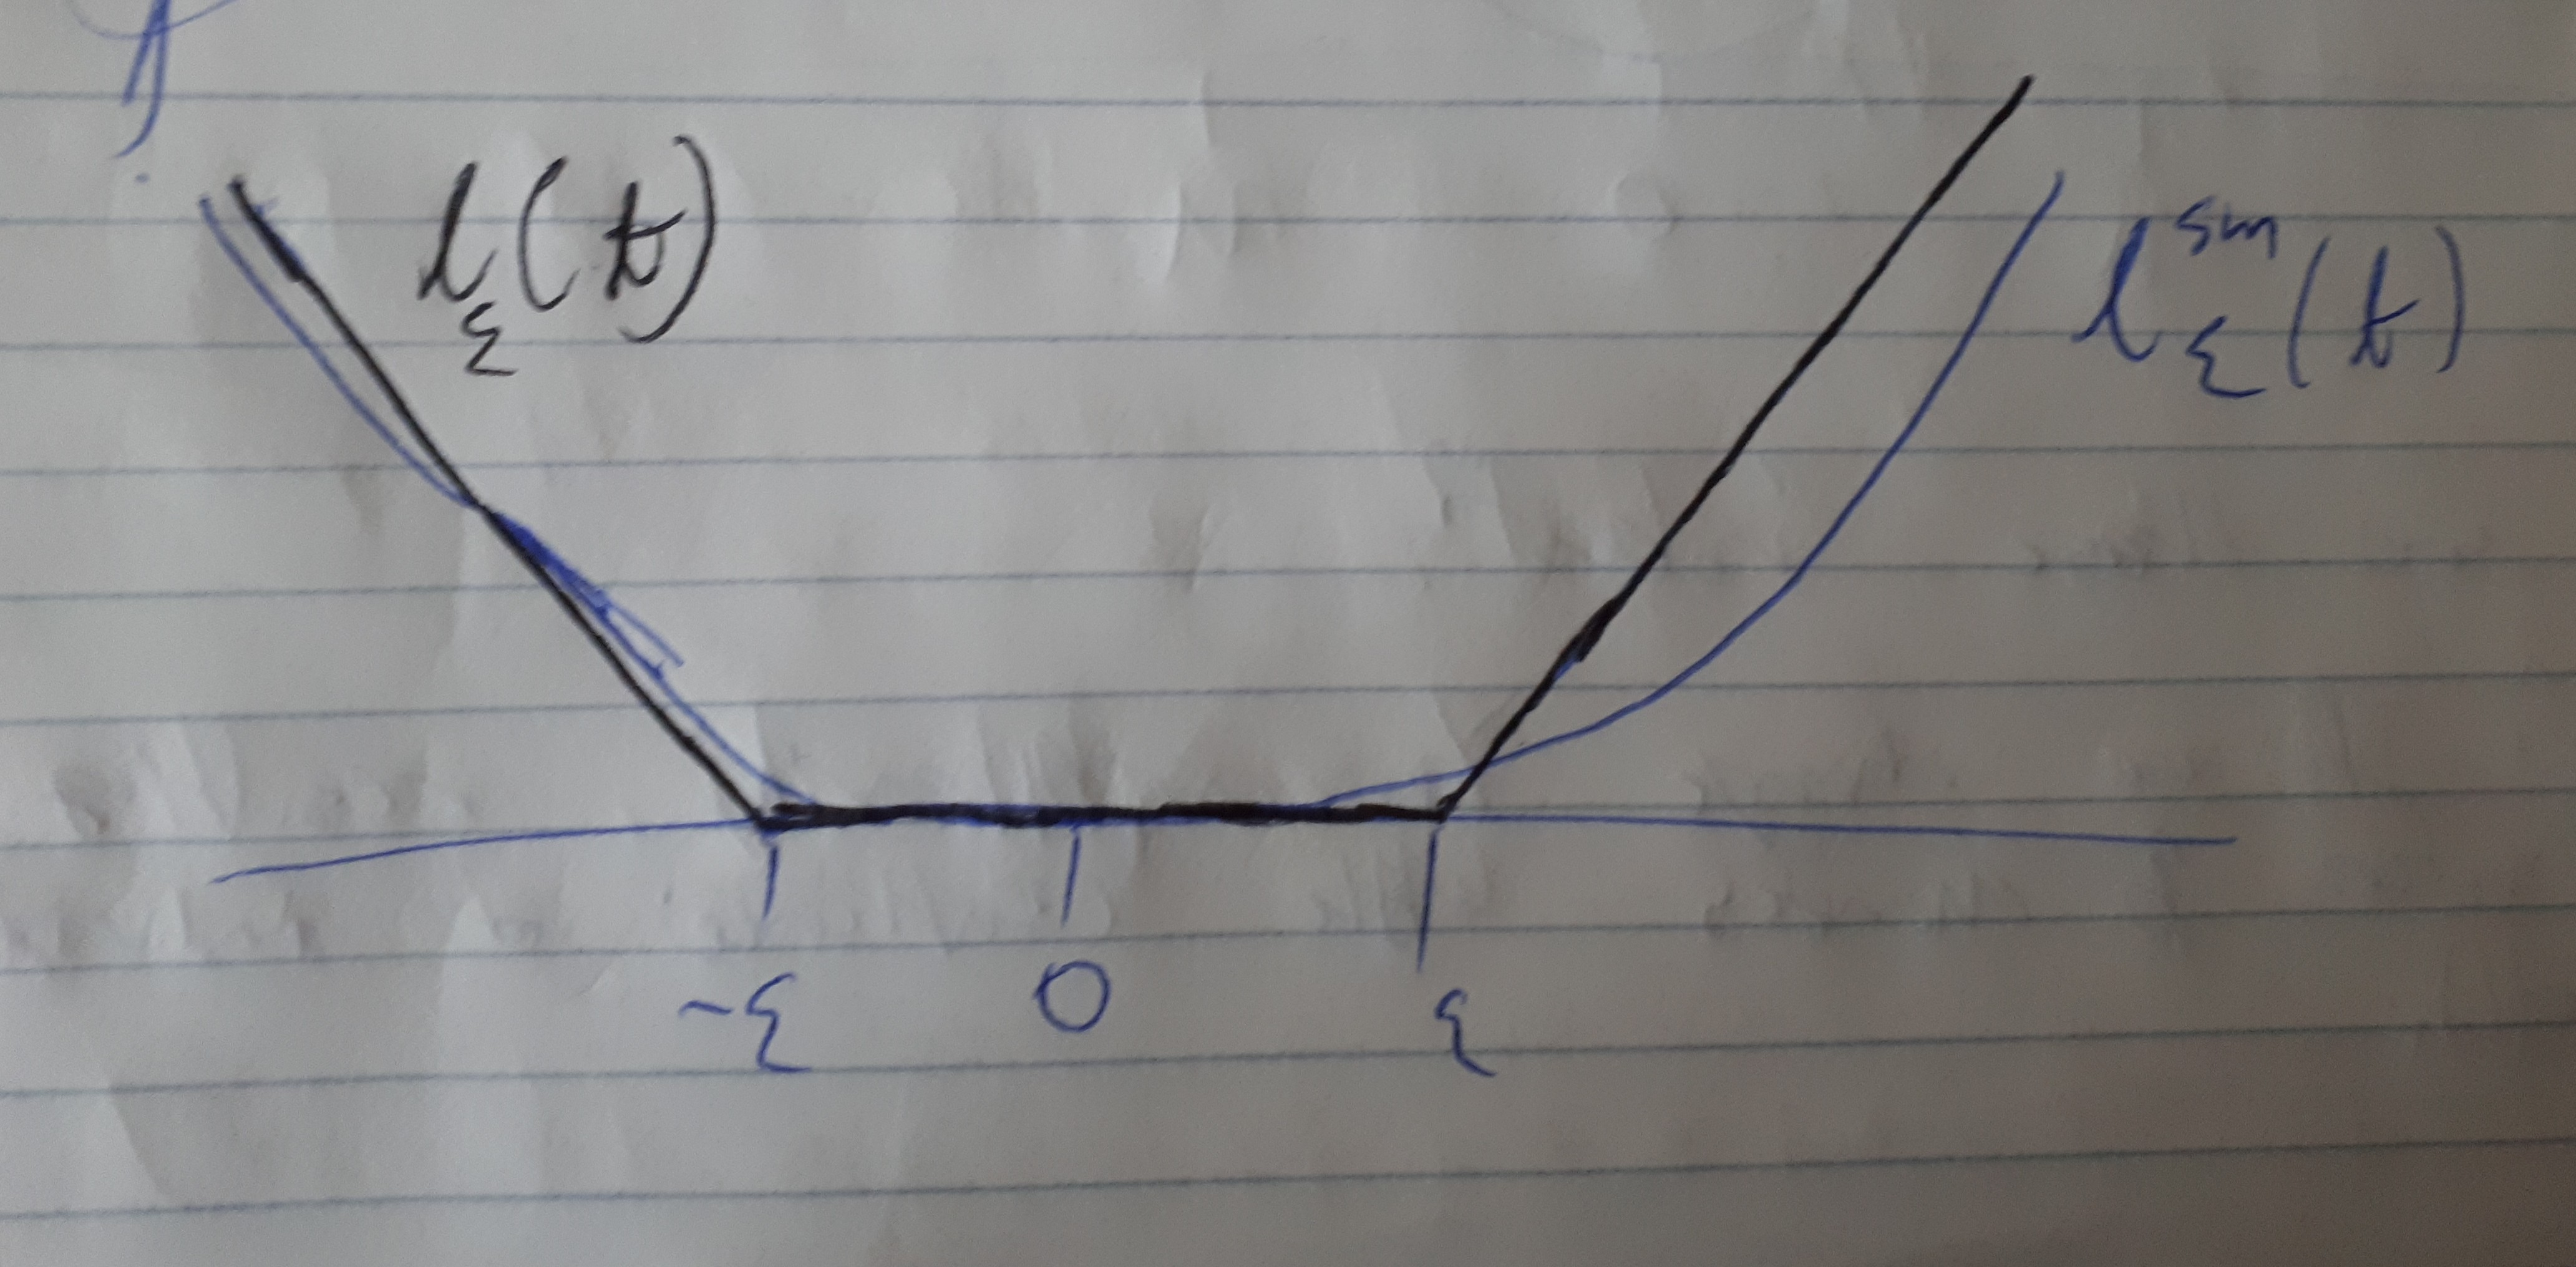
\includegraphics[width = 0.7\textwidth]{11_18_P03.jpg}
    \end{center}
    \item \emph{Smoothed $\eps$-insensitive loss} is a smooth version of $\eps$-insensitive loss. It is defined by:
    \[l_\eps^{sm}(t) = \log(1+\exp(t-\eps))+\log(1+\exp(-t-\eps)).\]
    This is the blue function in the picture above. We also have rescaled versions of the smoothed $\eps$-insensitive loss. For $a > 0$ define, 
    \[l^{sm}_{\eps,a}(t) = a \cdot l_\eps^{sm}\left(\frac{t}{a}\right),\]
    which satisfies \[\lim_{a \searrow 0} l_{\eps,a}^{sm}(t)=l_\eps(t).\]
    \item \emph{Huber loss}: for $u > 0$, define
    \[l(t) = \begin{cases}
        \frac{1}{2u} t^2 & \text{if } \abs{t} \le u,\\
        \abs{t}-\frac{u}{2} & \text{if } \abs{t} \ge u.
    \end{cases} \]
    Huber loss looks like this:
    \begin{center}
        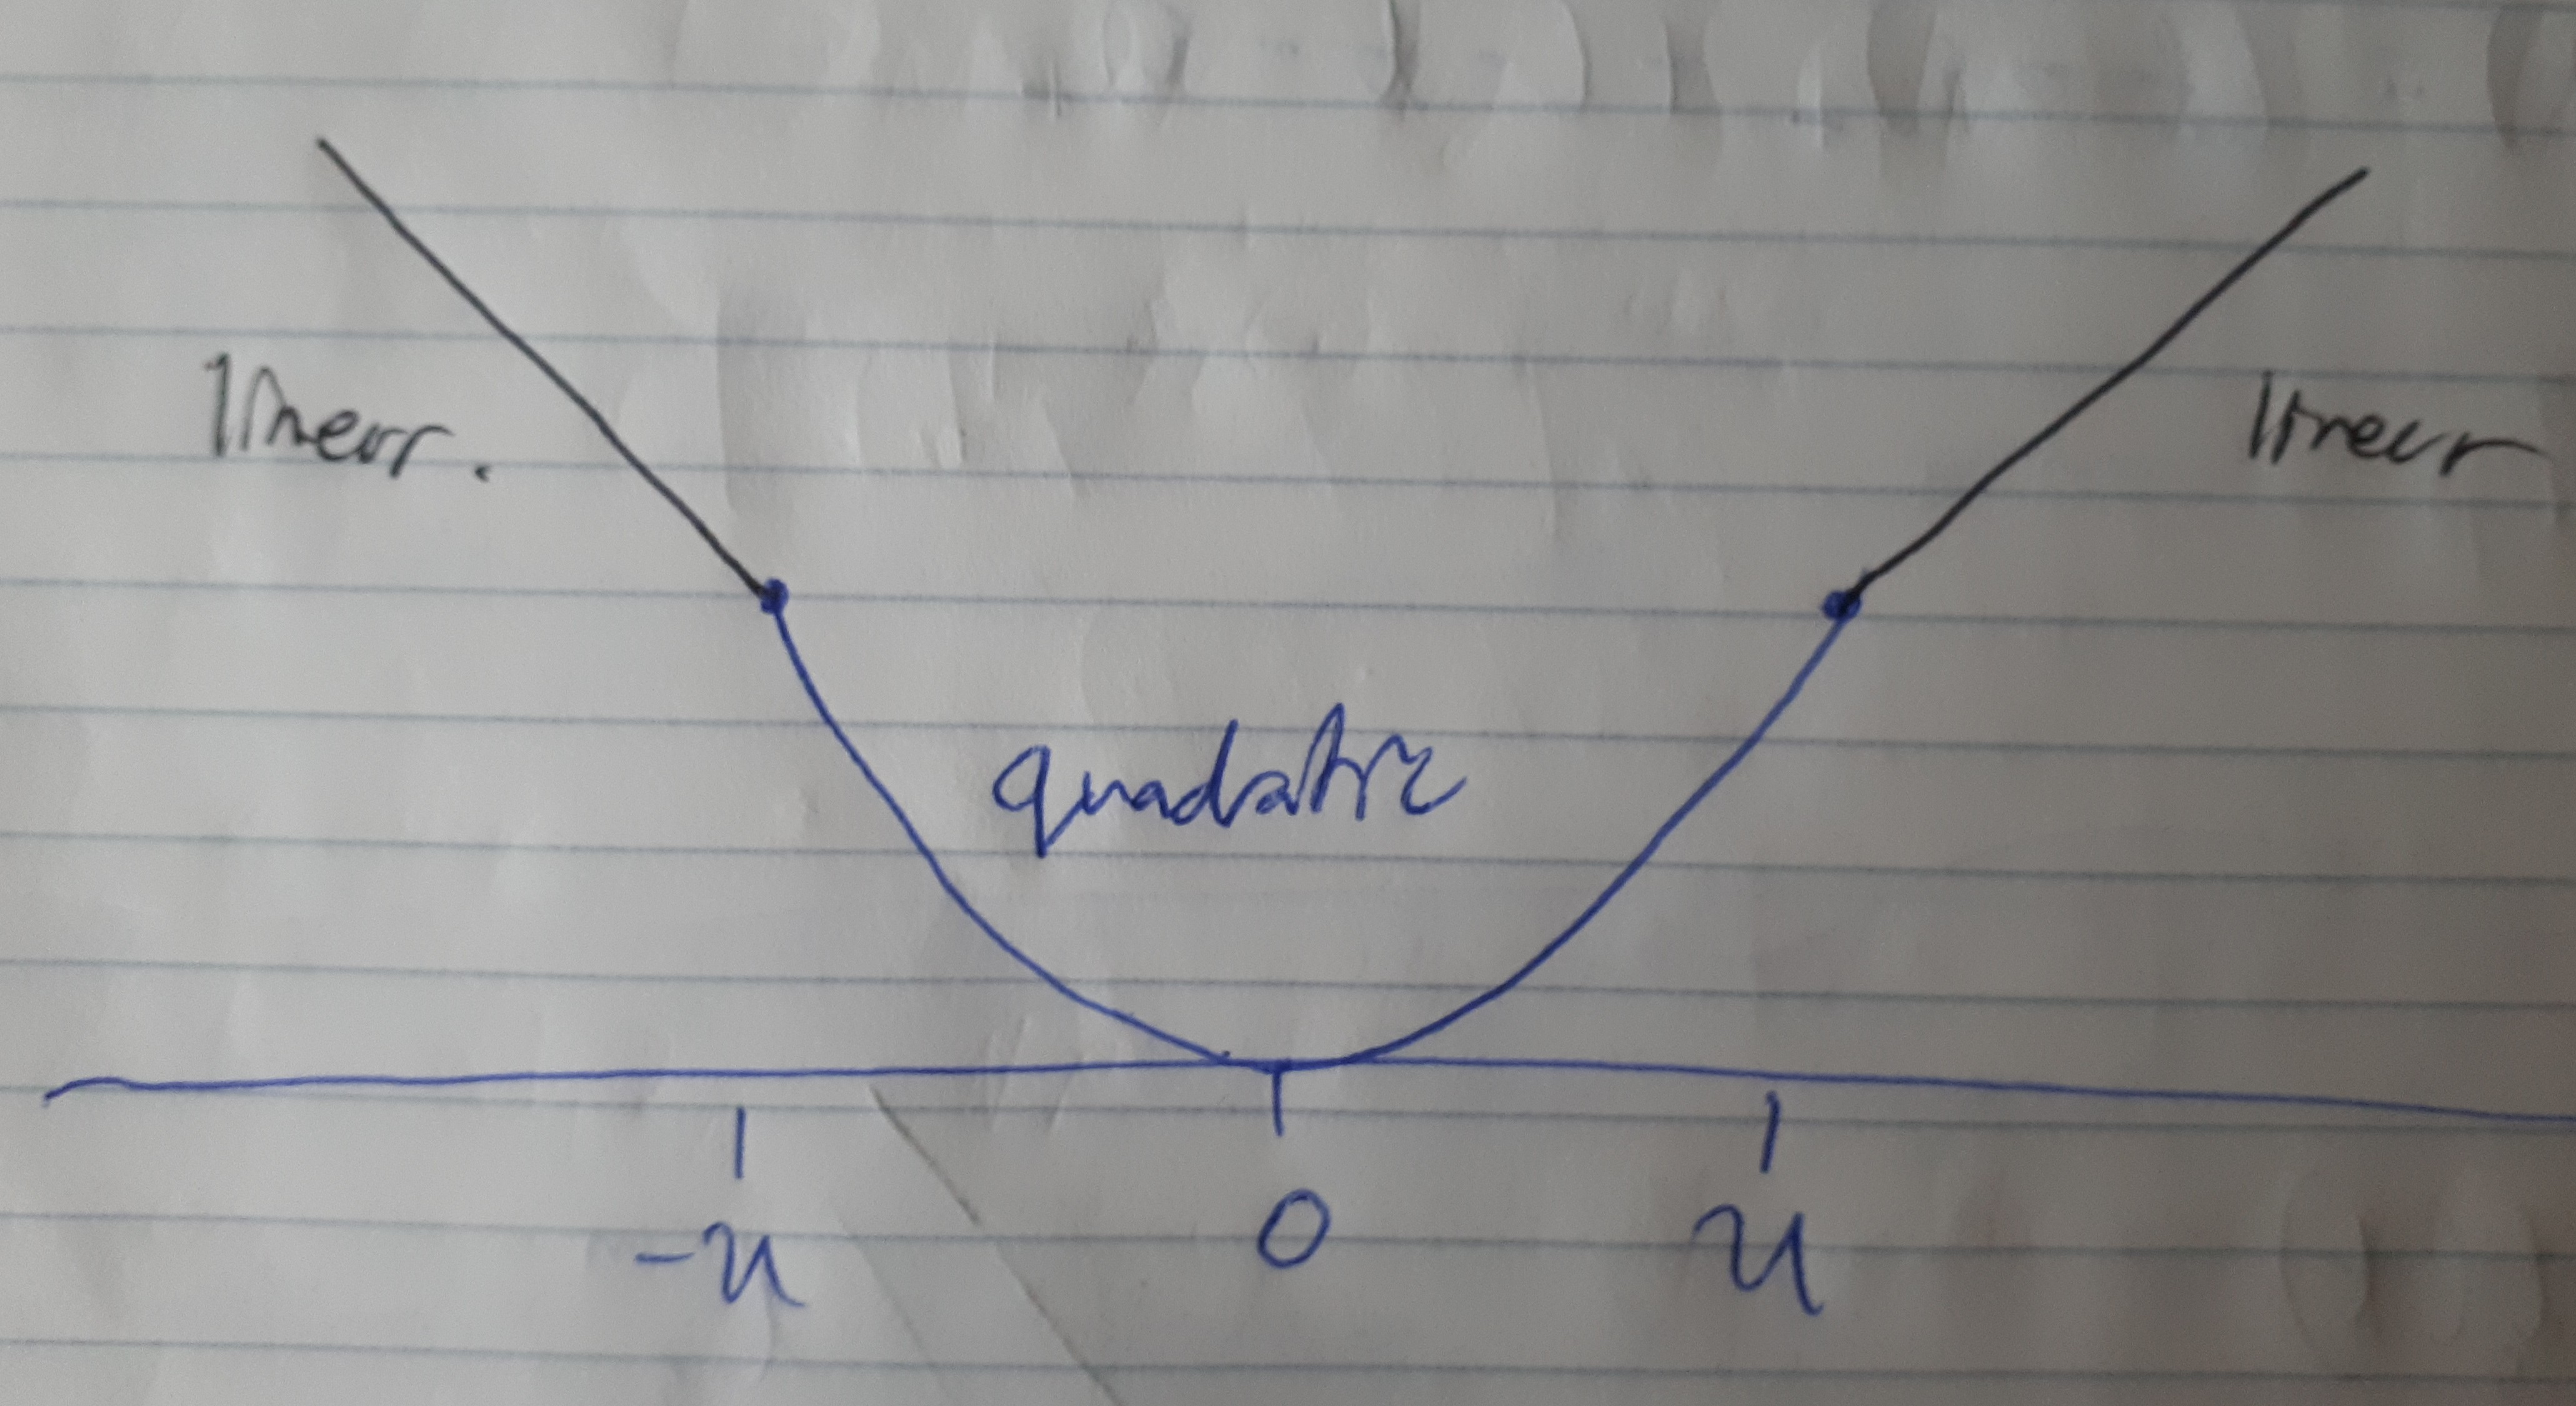
\includegraphics[width = 0.7\textwidth]{11_18_P04.jpg}
    \end{center}
\end{itemize}
Why are these M-estimators more ``robust''? The rough idea is that if we change a single $y_i$ arbitrarily, then the resulting estimator $\wh{\beta}$ changes little. Thus the influence of individual observations is small.

Some loss functions give estimators with this property, others do not. For example, we have seen that under squared error, points with high leverage can have a large influence on the model. 

It turns out that two things are key for an M-estimator to be robust:
\begin{itemize}
    \item The features $X_i$ are bounded.
    \item The loss function is (1)-Lipschitz. That is for all $t,s \in \R$, $\abs{l(t)-l(s)}\le {t-s}$ or equivialently $\abs{l'(t)}\le 1$ for all $t\in \R$.
\end{itemize}
This will be discussed more later and will be explored on upcoming homework.
\end{document}